\chapterimage{OCSDHeadworksScrubbersBW.jpg}
\chapter{Odor Control}

\section{Drivers for Odor Control}\index{Drivers for Odor Control}
\begin{enumerate}
\item Air Quality Regulations:\\
SCAQMD may issue a Notice of Violation (NOV) against the source of nuisance odors for creating a public nuisance, in violation of SCAQMD Rule 402 and California Health and Safety Code Section 41700.\\
\item Low Odor Thresholds:\\
Many of the compounds commonly found in wastewater such as H2S, skatoles have perceptible odors even at very low concentrations at parts per billion levels (ppb).\\
\item Worker Safety:\\
Ventilation requirements—to protect workers form health hazard associated with compounds such as H2S and to comply with fire and explosion prevention related regulations including NFPA, will generate foul air requiring treatment prior to discharge.\\
\item Corrosion Prevention
Severe corrosion potential of wastewater conveyance and treatment infrastructure due to H2S conversion by bacteria to sulfuric acid.\\
\item Good Neighbor Policy:\\
As many treatment plants and elements of its wastewater collections systems are located in populated areas, agencies adopt odor control strategies at both to remain a good neighbor, treatment plants and its collections to ensure transparent coexistence  minimizing odor complaints  ensure peaceful co-existence agencies adopt be a good neighbor by minimizing odors as a part of the normal operation of the wastewater treatment facility. \\
\end{enumerate}

Odors associated with wastewater, result from the release of the following:
\begin{enumerate}
\item compounds which are originally discharged into the sewer – chemicals, wastes, or 
\item by products of biological and chemical reactions occurring in wastewater
\end{enumerate}

\begin{itemize}
	\item Hydrogen sulfide is the most common wastewater origin odorous compound
	\item it is produced in wastewater by the activity of sulfate reducing bacteria which live in the slime layer in the sewer pipes.  
	\item hydrogen sulfide characteristics:
	\begin{itemize}
		\item has an offensive smell
		\item it is highly toxic and has the potential to instantly kill  
		\item it is converted into highly corrosive sulfuric acid through microbiological activity in the wastewater systems.  
	\end{itemize}
Thus, the prevention or treatment of odors, in particular hydrogen sulfide provides benefits including:
	\begin{itemize}
		\item safety
		\item preventing public nuisance, and
		\item  corrosion prevention.\\
	\end{itemize}
\vspace{0.5cm}
\item Other common odor pollutants include
\begin{itemize}
\item organic compounds - these are typically associated with the foul air from the preliminary, primary and secondary treatment processes
\item ammonia - the odor causing constituent of the foul air from dewatering operations associated with anaerobic digested sludge.\\
\end{itemize}
\end{itemize}
\vspace{0.5cm}
Odor control is applied to both - liquid and air phases. Odor control options for both - vapor and liquid phase treatments, are summarized below.


\begin{figure}
	\begin{center}
		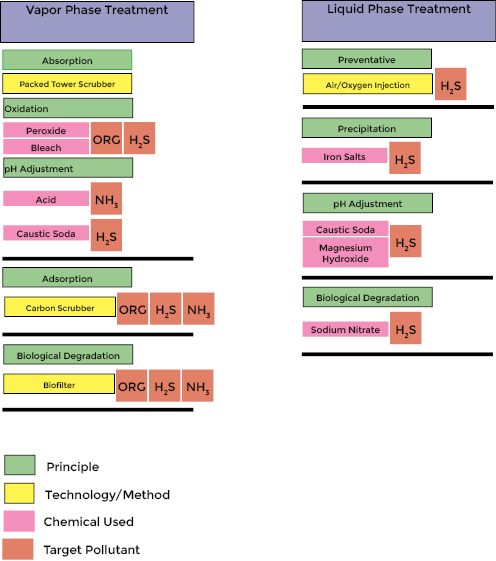
\includegraphics[scale=.82]{OdorControl}
			\caption{Odor Control Options}
	\end{center}
	
	\end{figure}

\section{Liquid Phase Odor Control Methods}\index{Liquid Phase Odor Control Methods}
\begin{itemize}
	\item typically applied in the collections systems
	\item goal for this treatment is to prevent nuisance odors associated with the production and release of hydrogen sulfide
	\item strategies include:
		\begin{itemize}
			\item air/oxygen injection - this prevents developing anaerobic condition and thus  formation of hydrogen sulfide
			\item iron salts react with the hydrogen sulfide present in the wastewater to form insoluble iron sulfide precipitate
			\item addition of alkaline chemicals including caustic soda or magnesium hydroxide increases the pH of the wastewater, preventing the escape of the hydrogen sulfide to the air phase as under alkaline condition H$_2$S is present as HS$^-$.  Caustic soda also helps remove the slime layer in the collections piping where the anaerobic bacteria responsible for the formation of hydrogen sulfide are present.  Magnesium hydroxide is used primarily because of it being environmentally safer and its reaction with hydrogen sulfide to form polysulfides
			\item Addition of sodium nitrate (Trade Name - Bioxide) promotes the activity of certain bacteria such as \textit{Thiobacillus denitrificans}, typically present in wastewater, which oxidize reduced sulfur compounds (like $H_2S$) while denitrifying the nitrate.  Presence of nitrate, also, increases oxidation-reduction potential, inhibiting the production of any odorous compounds such as hydrogen sulfide which are produced under anaerobic conditions.
		\end{itemize} 
\end{itemize}


\section{Vapor Phase Odor Control Methods}\index{Vapor Phase Odor Control Methods}
\begin{itemize}
	\item is typically applied inside the plant
	\item foul air from the treatment processes is captured and scrubbed using either a packed tower scrubber, a carbon scrubber or a biofilter.
	\begin{itemize}
		\item Packed Tower Scrubber - This involves spraying of a recirculated liquor from the top with the foul air injected from the bottom.  The plastic packing media provides the surface to facilitate the transfer of the soluble pollutants from the air phase to the liquid phase.  The pollutant transferred to the liquid phase has to be chemically or biologically removed and the recirculation water has to be wasted periodically to prevent the build-up of the pollutant in the recirculation water.

A schematic cross section of a packed tower scrubber is provided below.

\begin{figure}
	\begin{center}
		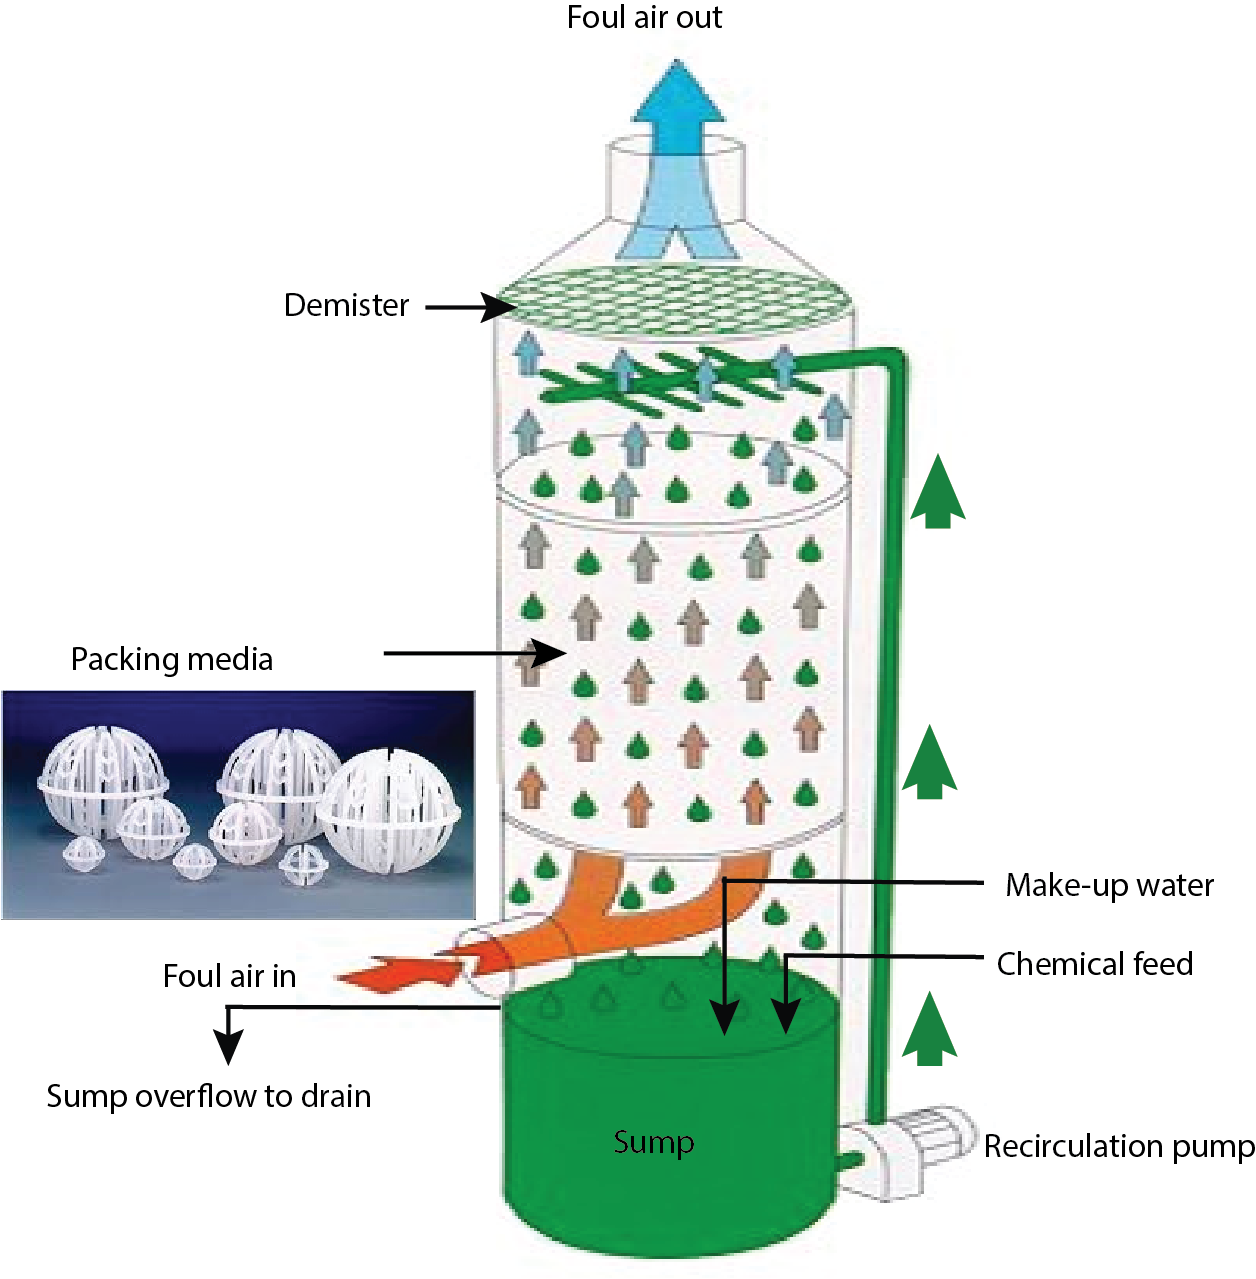
\includegraphics[scale=1.6]{OdorPackedTowerScrubber1}
			\caption{Packed Tower Scrubber}
	\end{center}
	
	\end{figure}
		\begin{itemize}
			\item for controlling organics - an oxidant such as hydrogen peroxide or bleach is added to recirculation water.  Organics control is typically exercised for foul air from the preliminary and secondary treatment processes.
			\item for controlling hydrogen sulfide - oxidants including hydrogen peroxide and bleach are utilized.  Additionally alkaline chemicals such as caustic soda or bleach (which is a solution of sodium hypoclorite in caustic soda) ionize the hydrogen sulfide thus stabilizing it (preventing its escape back into the air phase)


\begin{figure}
	\begin{center}
		\includegraphics[scale=0.3]{OdorH2Sequilibrium}
			\caption{H$_2$S - H$_2S^-$ pH Equilibrium Curve}
	\end{center}
	
	\end{figure}
	
\begin{figure}
	\begin{center}
		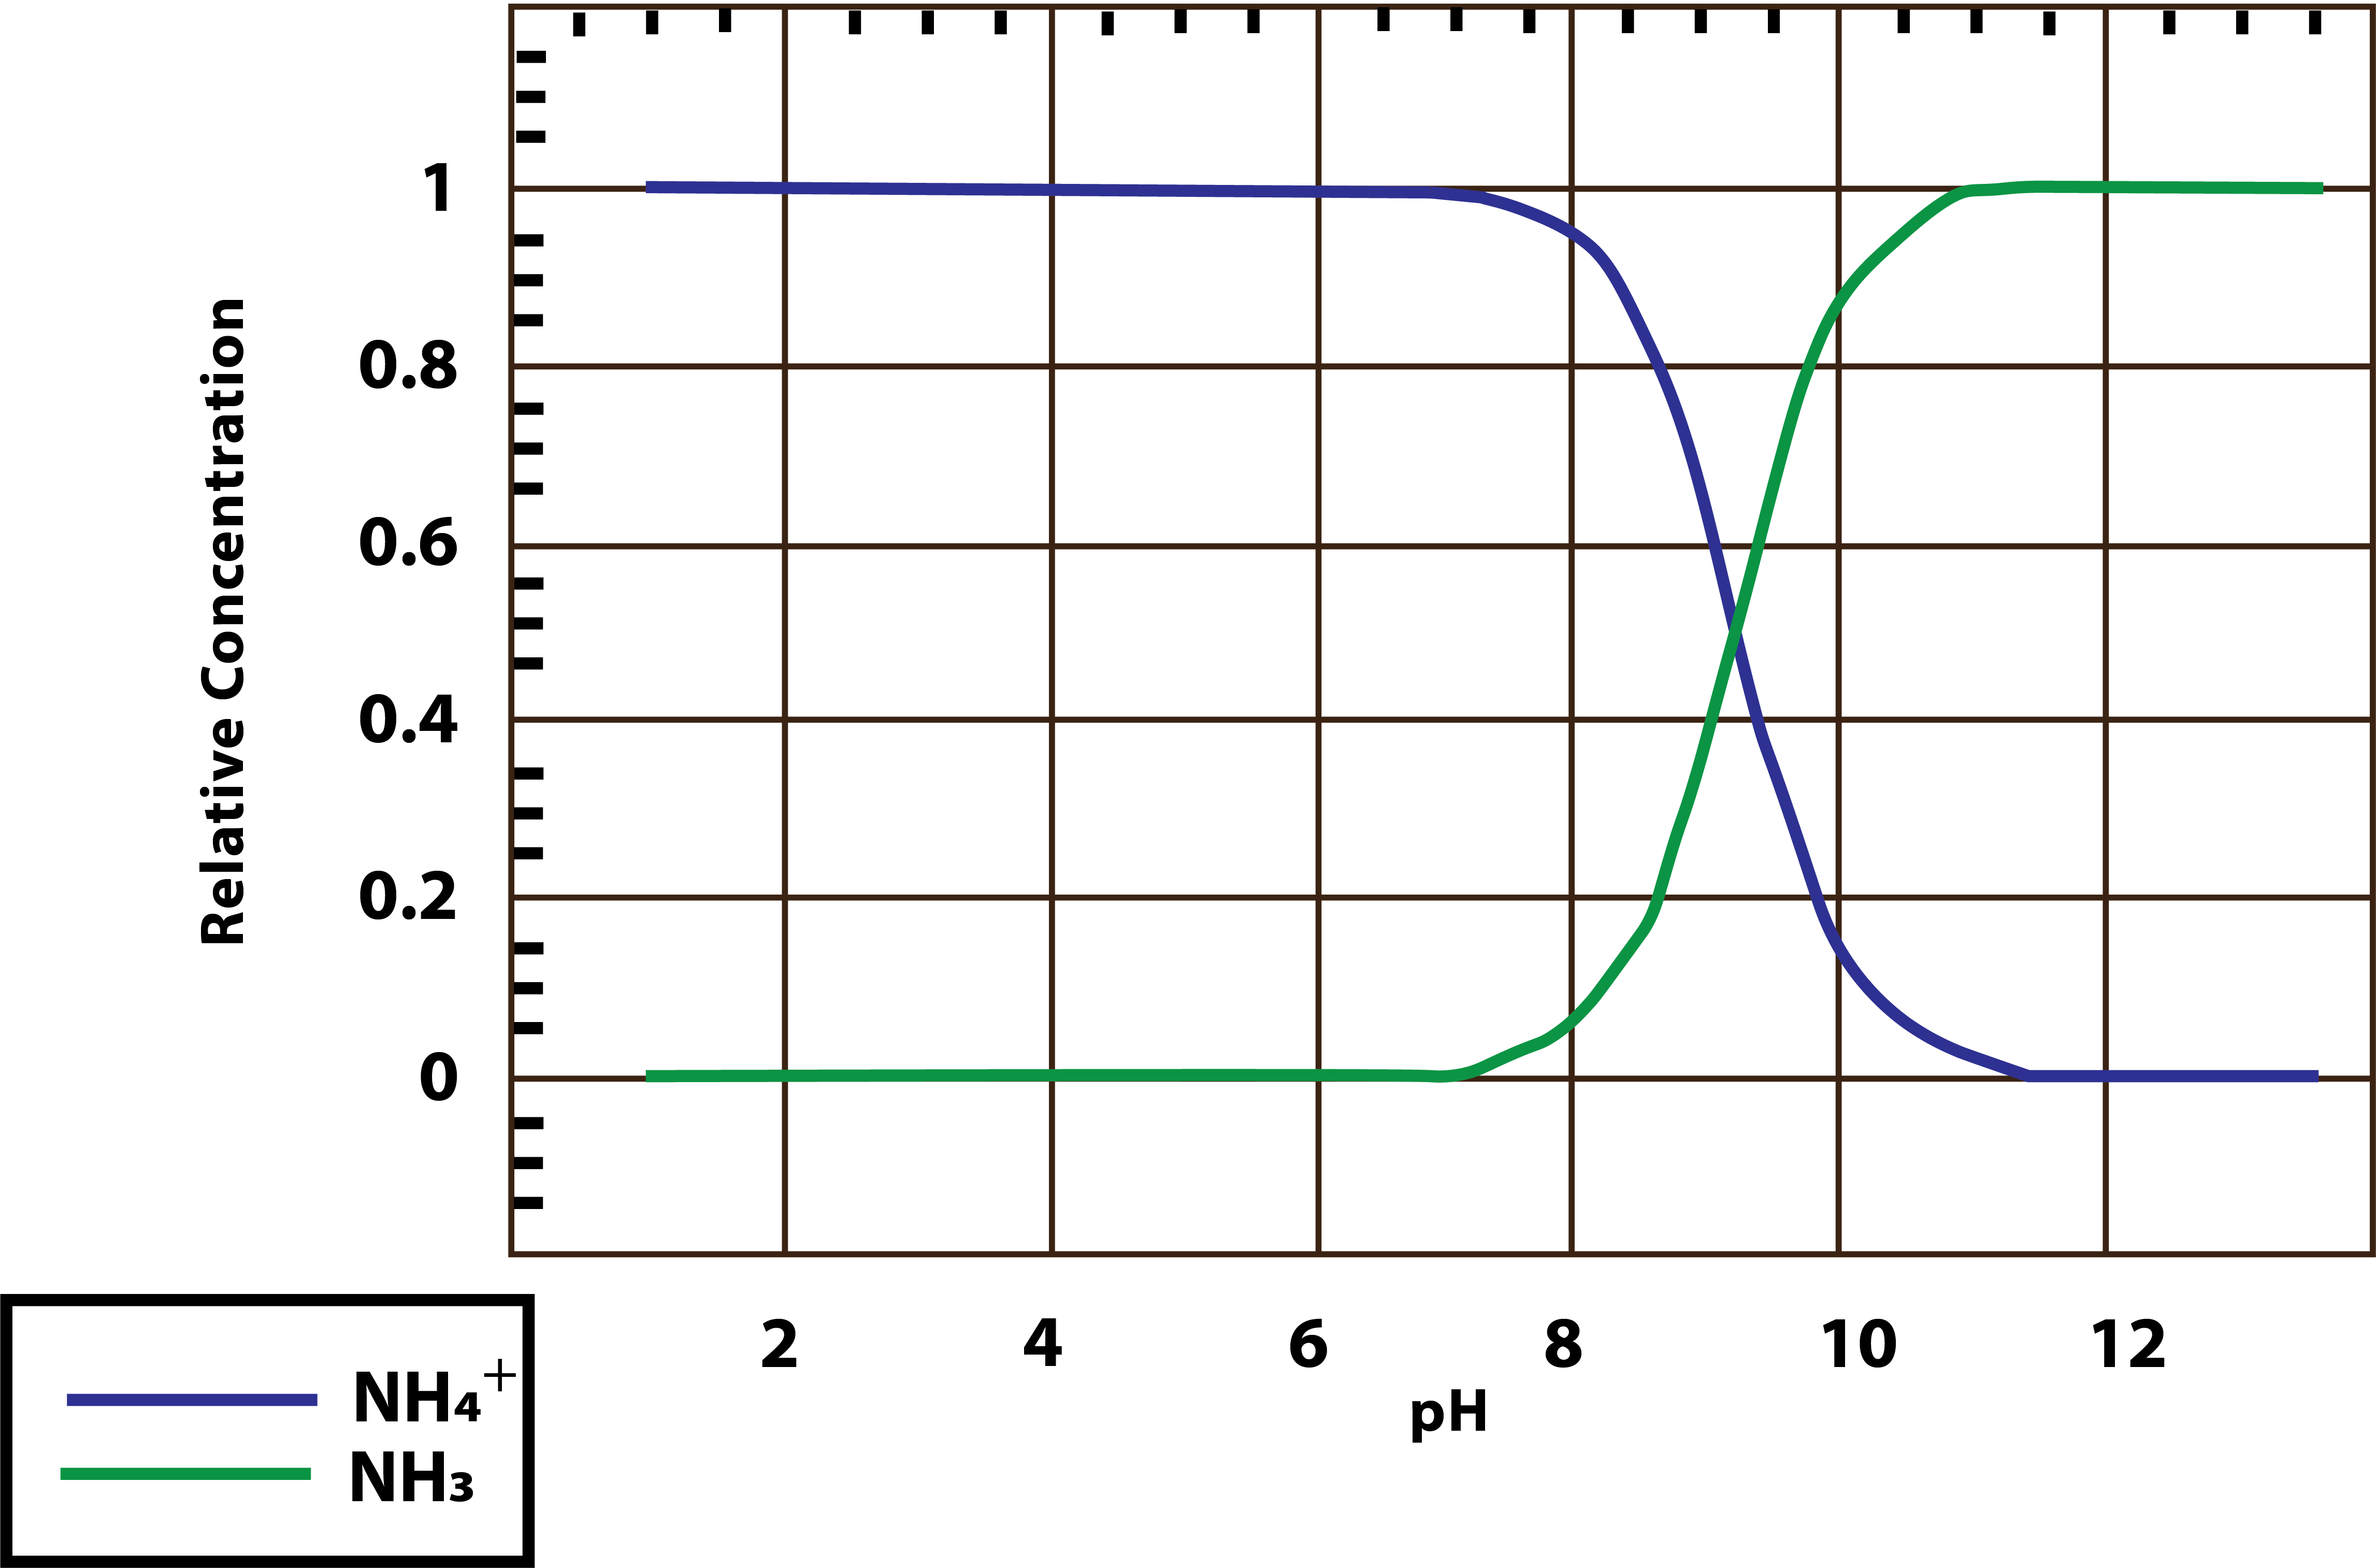
\includegraphics[scale=0.25]{AmmoniaAmmoniumEquilibrium}
			\caption{NH$_3$ - NH$_4^+$ pH Equilibrium Curve}
	\end{center}
	
	\end{figure}	


			\item for controlling ammonia - due to high solubility of ammonia, just water without any chemicals may be used.  If the concentration of ammonia is higher, an acid may be added to the recirculation water to keep the ammonia ionized.

The packed tower scrubber may be used in a biological treatment mode - as a biotrickling filter, where a microbiological population which feed on the dissolved pollutants is allowed to develop. 
 	\end{itemize}
 		\item Biofilters involve use of microorganisms growing on a slime layer on a packed substrate - biofilter media.  The pollutants from the foul air dissolve in the slime layer as it passes through the biofilter.  Once in the slime layer, the pollutant are consumed by the microbes.  In order to maintain the slime layer and prevent the biofilter from drying out, the biofilter is irrigated periodically and/or the foul air stream is humidified.  The substrate can be a organic or inert material including compost or activated carbon.  A typical cross-section of a biofilter is shown below


\begin{figure}
	\begin{center}
		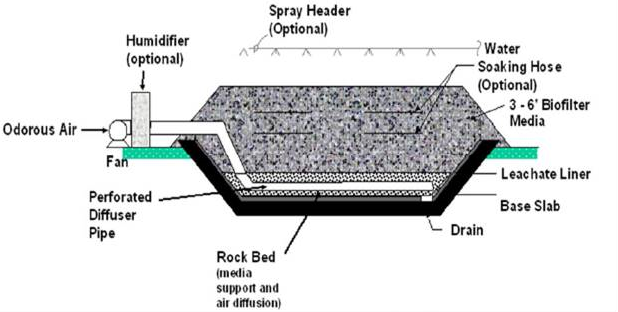
\includegraphics[scale=0.8]{Biofilter}
			\caption{Biofilter}
	\end{center}
	
	\end{figure}

		\item Carbon scrubber is comprised of a  packed bed of specially produced carbon pellets which have an active surface area which adsorb the pollutants from the foul air stream passing through it. The carbon may be impregnated with an oxidant such as potassium permanganate or a alkaline substrate to enhance its effectiveness in treating foul air with organics and hydrogen sulfide respectively.
\end{itemize}
\end{itemize}


